\chapter{Affine Spaces and Vectors: A Geometric Foundation}

We view calculus as a fundamental tool for understanding geometry. To begin this journey, we must first discuss the basic notions of geometry that will serve as our foundation. This chapter focuses on the geometry of $\mathbb{R}^n$, providing essential intuition about its structure and offering a modern perspective on the nature of geometry itself.

\section[From High School Geometry to University Mathematics]{From High School Geometry to University Mathematics}

In this chapter we study some very basic concepts in high-dimensional geometry. Why do we consider geometry at all, if our main goal is to study calculus? In the calculus of a single variable, geometric intuition plays a crucial role. We understand the derivative as the slope of a tangent line, and the integral as the area under a curve. These geometric interpretations provide a mental map that guides us through formal proofs and calculations.

As we move to the calculus of several variables, we wish to retain this powerful advantage. We want to be able to use our geometric intuition to navigate the analysis of functions in higher dimensions. However, our innate intuition is limited to three dimensions. To work effectively in $\mathbb{R}^n$, we must therefore extend our geometric instincts. We do this by taking familiar concepts from the plane and space—such as points, vectors, lines, and distances—and generalizing them to $n$ dimensions.

This chapter is dedicated to establishing this geometric foundation. Our primary aim is to harness our low-dimensional intuition to make high-dimensional calculus natural and accessible. However, as we progress, we will discover that the relationship between these fields is two-way. Just as geometry provides intuition for calculus, the powerful tools of calculus will ultimately allow us to explore and understand the geometry of high-dimensional spaces with a depth that intuition alone cannot provide.

When studying geometry in high school we distinguish between the intrinsic properties of a geometric object, and its specific location in space. We intuitively understand that a triangle remains the ``same'' triangle, and a circle the ``same'' circle, regardless of where they are located. On the other hand, when we ask questions about the relation within a collection of objects, for example whether a circle is contained in a triangle, then their relative position matters, and moving just one of them might change the answer. A familiar example of this principle is in the treatment of vectors: a vector can be represented as an ordered pair of points, an anchor point and a head, which together form an arrow shape starting at the anchor point and ending at the head. Two arrows are considered equivalent if they possess the same length and direction, even if they are anchored at different points. This discussion suggests that geometry is not about points or sets of points in space, but rather about the relationships between them, which are invariant under translations and perhaps also other operations.

In this chapter, we formalize this intuition and genralize it from the familiar setting of $\mathbb{R}^2$ and $\mathbb{R}^3$ to the general setting of $\mathbb{R}^n$. Indeed throughout this book we often use the familiar settings of $\mathbb{R}^2$ and $\mathbb{R}^3$ to illustrate concepts, while defining them in the general setting of $\mathbb{R}^n$. However to really start from the basics, we will begin with the simplest case of all, the one-dimensional space $\mathbb{R}^1$.


\section{Points and Translations in $\mathbb{R}^n$}

\subsection{The Space $\mathbb{R}^n$}
In elementary geometry, we represent points in the plane or in space using Cartesian coordinates. A point in the plane is uniquely identified by a pair of real numbers $(x, y) \in \mathbb{R}^2$, and a point in space by a triple $(x, y, z) \in \mathbb{R}^3$. This allows us to think of geometry as the study of the properties and relationships of these tuples of real numbers.

\begin{center}
\begin{tikzpicture}[scale=1, >=stealth]
  % 2D Point
  \draw[->] (-0.5,0) -- (2.5,0) node[right] {$x$};
  \draw[->] (0,-0.5) -- (0,2.5) node[above] {$y$};
  \fill (1,1) circle (2pt) node[above right] {$(1,1)$};
\end{tikzpicture}
\hspace{1.5cm}
\begin{tikzpicture}[scale=1, >=stealth]
%TODO: finish this illustration
  \draw[->] (-0.5,0,0) -- (2.5,0,0) node[right] {$x$};
  \draw[->] (0,-0.5,0) -- (0,2.5,0) node[above] {$y$};
  \draw[->] (0,0,-0.5) -- (0,0,2.5) node[above] {$z$};
  \fill (1,1,1) circle (2pt) node[above right] {$(1,1,1)$};
\end{tikzpicture}
\end{center}

We can extend this idea to any dimension $n$ by defining the space $\mathbb{R}^n$ as the set of all $n$-tuples of real numbers:
\[ \mathbb{R}^n = \{ (x_1, \dots, x_n) \mid x_i \in \mathbb{R} \} \]
While our direct intuition is rooted in $\mathbb{R}^2$ and $\mathbb{R}^3$, we can carry these algebraic structures over to $\mathbb{R}^n$, allowing us to study geometry in higher dimensions. Elements of $\mathbb{R}^n$ are called both \textbf{points} and \textbf{vectors}, reflecting the fact that they can be viewed either as locations in space (points) or as displacements from the origin (vectors).

\subsection{Vector Addition}
Given two vectors $x = (x_1, \dots, x_n)$ and $y = (y_1, \dots, y_n)$ in $\mathbb{R}^n$, we define their \textbf{sum} by adding corresponding components:
\[ x + y = (x_1 + y_1, \dots, x_n + y_n) \]
This operation is inherited from the component-wise structure of $\mathbb{R}^n$ and satisfies familiar properties such as commutativity ($x+y = y+x$) and associativity ($(x+y)+z = x+(y+z)$).

\subsection{Translations (Shifts)}
A fundamental operation in this space is moving from one point to another.
Given a fixed vector $y \in \mathbb{R}^n$, we define the \textbf{translation} (or shift) map $S_y: \mathbb{R}^n \to \mathbb{R}^n$ by:
\[ S_y(x) = x + y \]
where the sum $x+y$ is the vector addition defined above.
Intuitively, this map shifts the entire space by the vector $y$.
If $K \subseteq \mathbb{R}^n$ is a shape, its translation is:
\[ S_y(K) = \{ x+y \mid x \in K \} \]
We denote this simply as $K+y$.


\section{Shapes as Equivalence Classes}

\subsection{Motivating the Concept of Shape}
When we think about geometry, we often want to discuss ``shapes'' in $\mathbb{R}^n$. A first attempt at formalizing this concept is to say that a shape is simply a subset of $\mathbb{R}^n$.

For example, the circle of radius 1 centered at the origin in $\mathbb{R}^2$ can be defined as:
\[ C_0 = \{ (x, y) \in \mathbb{R}^2 \mid x^2 + y^2 = 1 \} \]

But here's a question: what about the circle of radius 1 centered at the point $(2, 1)$?
\[ C_{(2,1)} = \{ (x, y) \in \mathbb{R}^2 \mid (x-2)^2 + (y-1)^2 = 1 \} \]

Are these two different shapes? Intuitively, they are the \textit{same} shape—a circle of radius 1—just positioned at different locations. We don't want the location to matter when defining what a ``shape'' is.

\subsection{Congruence by Translation}
To formalize the idea that $C_0$ and $C_{(2,1)}$ are the ``same shape,'' we introduce the notion of \textbf{congruence by translation}.

Two subsets $K, L \subseteq \mathbb{R}^n$ are said to be \textbf{congruent by translation} (denoted $K \cong_T L$) if there exists a vector $y \in \mathbb{R}^n$ such that $K+y = L$.

This connects to high school geometry: two shapes are ``congruent'' if you can pick one up and place it on top of the other. In this context, we restrict to pure translation (no rotation).

\textbf{Example:} The two circles $C_0$ and $C_{(2,1)}$ are congruent by translation. Indeed, if we translate $C_0$ by the vector $y = (2, 1)$, we get:
\[ C_0 + (2,1) = \{ (a+2, b+1) \mid a^2 + b^2 = 1 \} = \{ (u, v) \mid (u-2)^2 + (v-1)^2 = 1 \} = C_{(2,1)} \]

\subsection{Shapes as Equivalence Classes of Sets}
Congruence by translation is an equivalence relation on the collection of subsets of $\mathbb{R}^n$.

\textbf{Exercise:} Verify that $\cong_T$ is reflexive, symmetric, and transitive. (Hint: Use properties of vector addition. This follows the same pattern as the arrow equivalence relation we prove in Section 3.6.)

To make congruent sets count as the \textit{same} shape, we define a \textbf{shape} to be an equivalence class under this relation. That is, a shape is not a specific subset of $\mathbb{R}^n$, but rather a collection of all subsets that are congruent by translation to one another.

Under this definition, the circles $C_0$ and $C_{(2,1)}$ belong to the same equivalence class, so they represent the same shape: ``a circle of radius 1.''

\subsection{Generalizing to Tuples of Points}
The concept of congruence by translation can be generalized in an obvious way to tuples of points or even to tuples of sets. For instance, two pairs of points $(x_1, x_2)$ and $(y_1, y_2)$ could be considered congruent if there exists a translation $v$ such that $x_1 + v = y_1$ and $x_2 + v = y_2$.

This generalization is particularly useful when we want to study geometric objects that are defined not just by a single set, but by relationships between multiple points or sets.

\subsection{Arrows: A Useful Special Case}
A particularly important application of this idea is to \textbf{arrows}. In high school physics or geometry, we often draw ``arrows'' to represent vectors. An arrow has a starting point and an ending point.

Consider two points $x, z \in \mathbb{R}^n$. We can draw an arrow starting at $x$ and ending at $z$. Intuitively, we say that the arrow from $x$ to $z$ represents the same vector as the arrow from $x'$ to $z'$ if they are parallel and have the same length.

Mathematically, we can formalize this using the concept of congruence: two pairs of points $(x, z)$ and $(x', z')$ should be considered equivalent (represent the same arrow) if there exists a translation that maps $x$ to $x'$ and simultaneously maps $z$ to $z'$. This happens precisely when $z - x = z' - x'$.

\subsection{Formal Definition: Arrow Equivalence}
We define a relation $\sim$ on the set of pairs of points $\mathbb{R}^n \times \mathbb{R}^n$.
We say that $(x, z) \sim (x', z')$ if:
\[ z - x = z' - x' \]

This is an \textbf{equivalence relation} (it is reflexive, symmetric, and transitive).

\begin{proof}
We verify the three properties of an equivalence relation:
\begin{itemize}
    \item \textbf{Reflexivity:} For any pair $(x, z)$, we have $z - x = z - x$, so $(x, z) \sim (x, z)$.
    
    \item \textbf{Symmetry:} If $(x, z) \sim (x', z')$, then $z - x = z' - x'$. This implies $z' - x' = z - x$, so $(x', z') \sim (x, z)$.
    
    \item \textbf{Transitivity:} Suppose $(x, z) \sim (x', z')$ and $(x', z') \sim (x'', z'')$. Then $z - x = z' - x'$ and $z' - x' = z'' - x''$. By transitivity of equality, $z - x = z'' - x''$, so $(x, z) \sim (x'', z'')$.
\end{itemize}
\end{proof}

\textbf{Geometric Intuition:} The condition $z - x = z' - x'$ is equivalent to saying $z' - z = x' - x$, meaning the quadrilateral formed by points $x, z, z', x'$ is a parallelogram. This visually shows that the arrows have the same direction and length.

\begin{center}
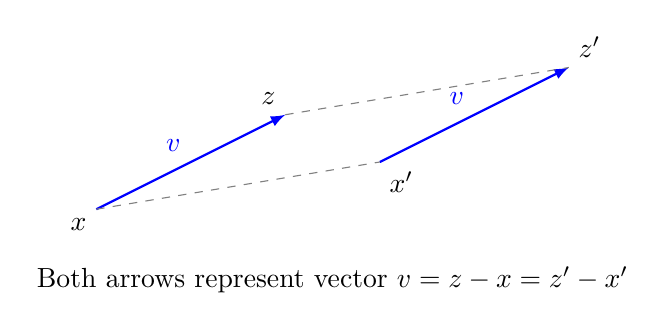
\begin{tikzpicture}[scale=1.2]
    % Define points
    \coordinate (x) at (0,0);
    \coordinate (z) at (2,1);
    \coordinate (xp) at (3,0.5);
    \coordinate (zp) at (5,1.5);
    
    % Draw arrows
    \draw[-latex, thick, blue] (x) -- (z) node[midway, above left] {$v$};
    \draw[-latex, thick, blue] (xp) -- (zp) node[midway, above left] {$v$};
    
    % Draw parallelogram
    \draw[dashed, gray] (x) -- (xp);
    \draw[dashed, gray] (z) -- (zp);
    
    % Label points
    \node[below left] at (x) {$x$};
    \node[above left] at (z) {$z$};
    \node[below right] at (xp) {$x'$};
    \node[above right] at (zp) {$z'$};
    
    % Show that both arrows represent the same vector
    \node[below] at (2.5, -0.5) {Both arrows represent vector $v = z - x = z' - x'$};
\end{tikzpicture}
\end{center}

We define an \textbf{arrow} to be an equivalence class under this relation.

\subsection{Representing Arrows}
An arrow (as an equivalence class of pairs of points) can be represented in two useful ways:

\textbf{1. As a vector in $\mathbb{R}^n$:} Each equivalence class corresponds to a unique displacement vector $v \in \mathbb{R}^n$. Specifically, the equivalence class of the pair $(0, v)$ contains all pairs $(x, z)$ such that $z-x = v-0 = v$. Thus, we can identify an arrow with the vector $v = z - x$ for any representative pair $(x, z)$ in its equivalence class.

\textbf{2. As a drawn arrow:} Each equivalence class can be visualized by drawing an actual arrow from any point $x$ to the point $z = x + v$. Different choices of starting point $x$ give different visual arrows, but they all represent the same equivalence class (the same ``abstract arrow'').

\subsection{Worked Example: Equivalent Arrows in \texorpdfstring{$\mathbb{R}^2$}{R2}}
Consider the following pairs of points in $\mathbb{R}^2$:
\begin{itemize}
    \item $(x_1, z_1) = ((1, 2), (4, 5))$
    \item $(x_2, z_2) = ((0, 0), (3, 3))$
    \item $(x_3, z_3) = ((-1, 1), (2, 4))$
\end{itemize}

We compute the displacement vectors:
\begin{align*}
z_1 - x_1 &= (4, 5) - (1, 2) = (3, 3) \\
z_2 - x_2 &= (3, 3) - (0, 0) = (3, 3) \\
z_3 - x_3 &= (2, 4) - (-1, 1) = (3, 3)
\end{align*}

Since all three pairs yield the same displacement vector $(3, 3)$, they all belong to the same equivalence class. They represent the same arrow, which can be identified with the vector $v = (3, 3)$, even though the actual drawn arrows start and end at different locations.


\section{Geometric Properties}
A property $\mathcal{P}$ of subsets of $\mathbb{R}^n$ is called a \textbf{geometric property} (with respect to translations) if it is invariant under translation.
That is, if a set $K$ has property $\mathcal{P}$, then for any shift $y$, the set $K+y$ also has property $\mathcal{P}$.
\textbf{Examples:}
\begin{itemize}
    \item ``Being a sphere'' is a geometric property.
    \item ``Containing the origin'' is \textbf{not} a geometric property (since shifting it might move the origin outside).
\end{itemize}
This formalism allows us to distinguish between intrinsic properties of a shape (like volume, shape type) and extrinsic properties (like position).


\section{Chapter Summary}

In this chapter, we established geometric foundations for $\mathbb{R}^n$ by formalizing intuitive notions of shapes, position, and vectors.

\textbf{Key Concepts:}
\begin{itemize}
    \item \textbf{Points and Vectors:} Elements of $\mathbb{R}^n$ can be viewed as locations (points) or displacements (vectors)
    \item \textbf{Vector Addition:} Component-wise sum $x+y = (x_1+y_1, \dots, x_n+y_n)$
    \item \textbf{Translation:} The map $S_y(x) = x + y$ shifts space by vector $y$
    \item \textbf{Congruence by Translation:} $K \cong_T L$ if $\exists y: K+y = L$
    \item \textbf{Shapes:} Defined as equivalence classes of congruent sets (position-independent)
    \item \textbf{Arrows:} Equivalence classes of pairs of points under $(x,z) \sim (x',z') \iff z-x = z'-x'$
    \item \textbf{Geometric Properties:} Properties invariant under translations
\end{itemize}

\textbf{Key Results:}
\begin{itemize}
    \item Congruence by translation is an equivalence relation
    \item Each arrow equivalence class corresponds to a unique displacement vector in $\mathbb{R}^n$
    \item Arrows can be represented as vectors or as drawn arrows
    \item Geometric properties distinguish intrinsic shape properties from extrinsic position properties
\end{itemize}

These concepts provide the foundation for Chapter 2 (norms and distances), Chapter 3 (O notation), and Chapter 4 (derivatives as linear approximations).

